\chapter{Neutrino  experiments}
\label{c:expIntro}

This chapter is aimed at putting the Baby MIND experiment into context of what has been done before, what experiments are under way and what experiments are planned.

\section{Neutrino detector experiments}

This section details some of the neutrino experiments that have and are taking place. The different experiments can be split into three different categories based on the primary neutrino source.
The detector types are:
\begin{itemize}
\item Accelerator
\item Atmospheric/Cosmic
\item Reactor
\end{itemize}
Each will be described briefly before examples are given.

\subsection{Accelerator}
Currently accelerator facilities can produce muon, electron both normal and anti neutrinos. This is done by starting with a hydrogen plasma, protons, which is then accelerated at a target to produce a shower of pions and muons. By using a magnetic horn these can be split by charge and then aimed at another target to provide muon neutrinos.

The other way is using the electrons which have been split from the hydrogen plasma and a similar method used to produce electron neutrinos.

The advantage of these neutrinos are that the energy range is well known and can be quite well tailored, the flux is huge compared to other methods. However the energy distribution will be quite wide because of the decay processes involved. It is also hard to produce a clean beam without background.

\subsubsection{K2K / T2-K}
After the success of Super-Kamiokande, the K2K-experiment\cite{22K2K} was created with the main difference of using a well understood muon neutrino beam pointing at the Super-Kamiokande detector at a distance of 250 km. It was the first neutrino oscillation measurement where both the source and detector were controlled, it observed the disappearance of muon neutrinos and found results that were consistent with Super-Kamiokande.

The next improvement came with the T2K-experiment\cite{21T2K}, which was also a long-baseline neutrino oscillation experiment with a more powerful beam from the JPARC facility to Super-Kamiokande, at a distance of 295 km. The experiment wanted to improve the understanding of the neutrino oscillation parameters. T2K was able to successfully observe the appearance of muon to electron neutrino oscillations and find evidence that the third mixing angle $\theta_{13}$ is not zero. This is still an ongoing experiment.

\subsubsection{MINOS}
MINOS~\cite{MINOS} is also a muon neutrino disappearance experiment, consisting of one near and one far detector and using the NuMI~\cite{19NuMI} beam at Fermilab, to better understand the neutrino beam and showed results consistent with Super-Kamiokande and the K2K experiments. This is one of the first MIND (Magnetised Iron Neutrino Detector) types build along with CDHSW \cite{40CDHSW}.

\subsubsection{NOvA}
After MINOS the next step using the NuMI~\cite{19NuMI} beam is the NOvA~\cite{18nova} experiment, which is also an electron neutrino appearance experiment and hopes to be able to determine the mass hierarchy of neutrinos.

\subsubsection{MINERvA}
The MINERvA (Main INjector ExpeRiment $\nu$-A)experiment \cite{39minerva} will also use the NuMI~\cite{19NuMI} beam to study neutrino-nucleus scattering to improve models of neutrino-nucleus scattering to reduce systematic uncertainties in results from oscillation experiments.

\subsubsection{MiniBooNE}
MiniBooNE\cite{41MiniBooNE} continued on what was started by MINOS but had the principle aim on improving neutrino mass measurements.

\subsection{Atmospheric/Cosmic}
For these experiments either solar, or other cosmological sources are used to provide the neutrinos. The main advantages are that the energy can be very high and it is possible to use the earth to remove all background providing an extremely clean signal.
However, it is impossible to control the source and difficult to get many events due to the low fluxes expected from astrophysical objects.

\subsubsection{SNO}
The Sudbury Neutrino Observatory (SNO)~\cite{Fix6} was build to make a definite measurement of solar neutrinos following on the measurements taken by the Homestake experiment~\cite{9Davis}. It consists of an 1000 ton heavy water detector 2 km underground. 

The experiment is currently replacing the heavy water with liquid scintilator and renaming it self as SNO+~\cite{42SNO+}.
\subsubsection{Super-K}
Super-Kamiokande\cite{20SUPERK}, an upgraded version of the Kamiokande water Cherenkov detector performed the first experimental observation that the neutrino has non-zero mass\cite{10Fukuda} and also managed to detect strong evidence of muon neutrino oscillation to tau neutrinos from the analysis of atmospheric neutrinos interacting in the water Cherenkov target.
\subsubsection{IceCube}
The IceCube observatory~\cite{43IceCube} uses the enormous detection volume of the South Pole to detect Cherenkov photons produced in the ice from neutrino interactions.
\subsection{Reactor}
For these experiments all neutrinos are provided through nuclear fission which means that the energy spectra of the neutrinos are well known and there is very little background. On the other hand the energy range is limited to be quite low compared to accelerator neutrinos.

\subsubsection{Double Chooz}
The Double Chooz experiment~\cite{45DoubleChooz} uses antineutrino to improve the neutrino mixing angle $\theta_{13}$ as well as showed that these detectors can be used to ensure non-proliferation.

\subsubsection{Daya Bay}
The Daya Bay experiment~ \cite{44DayaBay} main goal is to improve the measurement of $\theta_{13}$. It is improving results from Double Chooz. This is done by combining electron antineutrinos from eight identical detectors placed at three locations around the detector.

\subsubsection{KamLAND}
KamLAND, the Kamioka Liquide scintilator Anti-Neutrino Detector, was build in 2002 and helped investigate if there were any neutrino oscillations by looking at anti electron neutrinos emitted from distant reactors~\cite{46KamLAND}.

%\subsection{Summary of important discoveries}
%\textbf{Table, different mass and so on.}
%\subsection{Current limits}

\section{MIND detector}\label{subsec:MINDdetector}
Magnetized Iron Neutrino Detectors (MINDs) have been operated in several experiments such as MINOS~\cite{MINOS}.
This type of detector, with magnetized steel plates and scintillation plates, is well suited to provide large mass for neutrino experiments and is able to provide momentum measurements by using range and curvature calculations as well as providing charge identification. A MIND type detector has been selected as the baseline detector for a neutrino factory~\cite{ISS, 27Bross}, since it is the cheapest and most effective way of producing a large magnetized volume. This has provided the motivation for creating a prototype detector to perform a number of studies.

Since water Cherenkov and liquid argon detectors have been established or actively studied for future very large scale neutrino oscillation experiments, a MIND type detector is not foreseen to be used as the main interaction medium for any planned upcoming experiments.. A MIND type detector can however be used to provide charge identification of muons if positioned downstream of any neutrino target which is not magnetized.

\section{Future neutrino experiments}
%\subsection{KATRIN}

\subsection{Hyper-K}
The Hyper-Kamiokande Experiment\cite{24HyperK}  builds on the T2K-experiment\cite{21T2K} by improving the neutrino beam at JPARC, and building a 500 kton water Cherenkov detector, which aims to improve the sensitivity for $\delta_{cp}$.
\subsection{DUNE}
LBNF/DUNE\cite{23DUNE} is a new experiment aiming at looking at the full range of $\delta_{cp}$ with greater sensitivity than before by improving on the MINOS~\cite{MINOS} experiment, and performing an electron neutrino appearance measurement with a high-powered neutrino beam from Fermilab and a 40 kton liquid argon detector at a distance of 1300 km, in the Homestake mine in South Dakota.
\subsection{nuStorm experiment/Neutrino factory}
One concept to achieve a high number of neutrino events from a well-understood neutrino beam is the so called Neutrino Factory~\cite{25NUfact}, which will create a high number of electron and muon neutrino events from the decay of high-energy muons.

A nuSTORM facility, which could be seen as the first stage towards a neutrino factory, is expected to have sensitivity for sterile neutrinos with a MIND type detector \cite{29nuSTORM} upto 10$\sigma$ compared to previous measurements.
\begin{figure}[h!]
\centering
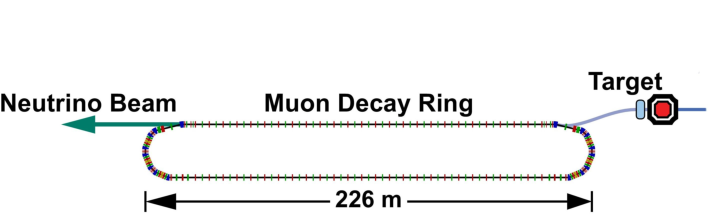
\includegraphics[width=\textwidth]{figures/nuSTORM_schematic.pdf}
\caption{A schematic of a nuSTORM facility~\cite{Fix7}.}
\label{fig:nuStorm}
\end{figure}

The neutrino factory has the capacity to improve the precision of neutrino oscillation measurements, since the neutrino beam from the decay of muons can be determined with high accuracy. The beam produces one bunch of $\mu^+$ and one bunch of $\mu^-$, so the facility can make measurements of $\nu_{\mu}$ and $\bar{\nu_{e}}$ and $\bar{\nu_{\mu}}$ and $\nu_{e}$ simultaneously. Using this $\delta_{cp}$ can be decisively explored, with an expected accuracy of $\Delta \delta_{CP}\sim 5^\circ$~\cite{25NUfact}.

\begin{figure}[h!]
\centering
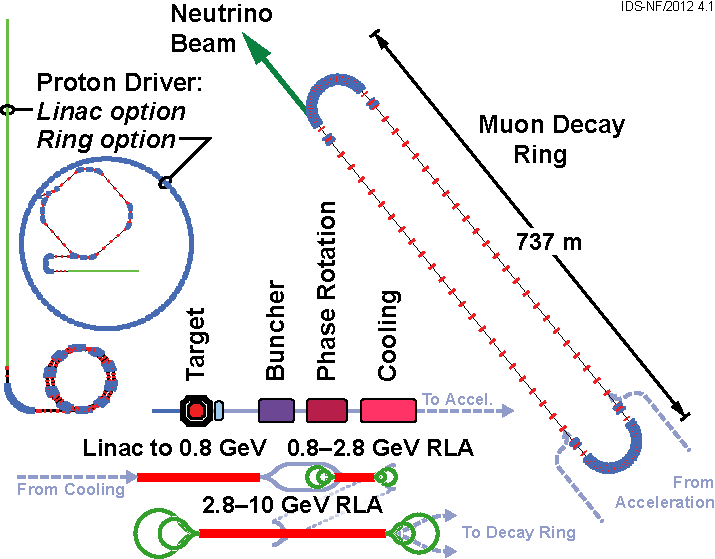
\includegraphics[width=0.9\textwidth]{figures/131112-IDS-NF.pdf}
\caption{Schematic diagram of the Neutrino Factory~\cite{Fix7}.}
\label{fig:nuFact}
\end{figure}

\begin{figure}[h!]
\centering
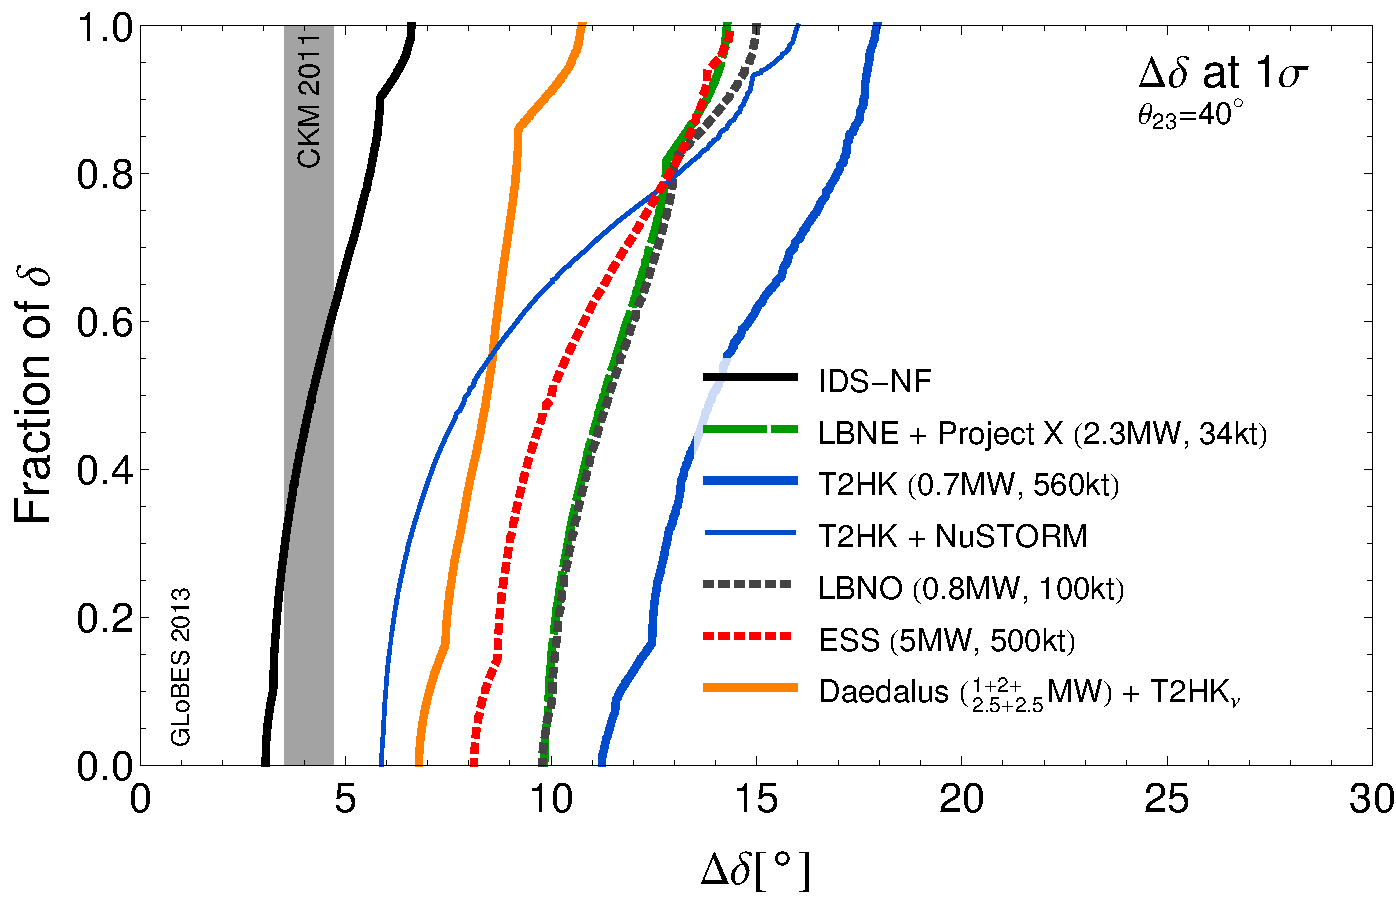
\includegraphics[width=0.9\textwidth]{figures/rdr-cp-precision-comparison-131216.pdf}
\caption{Expected precision for a measurement of the $\delta_{cp}$ at a Neutrino Factory compared to alternate neutrino oscillation facilities~\cite{Fix7}.}
\label{fig:nuFactExp}
\end{figure}

%==============================================================================
